\section{Estructura}
\begin{frame}
    \begin{columns}[t]
        \begin{column}{.5\textwidth}
          \tableofcontents[sections={1-2},currentsection]
        \end{column}
        \begin{column}{.5\textwidth}
          \tableofcontents[sections={3-4},currentsection]
        \end{column}
    \end{columns}
\end{frame}

\subsection{Moogle Server}
\begin{frame}[fragile]{Moogle Server}
Es donde se ha implementado la interfaz gráfica de la aplicación. En 
esta parte se ha agregado una línea en el archvio \textit{Program}
para cargar el repositorio antes de ejecutar la aplicación.

\pause

\begin{figure}
  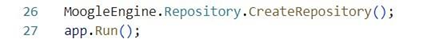
\includegraphics{img6.png}
\end{figure}


{\textit{\textbf{Importante:}}} El proyecto se ejecuta introduciendo el comando:
{\scriptsize\texttt{dotnet watch run --project MoogleServer}} en la terminal, desde la 
carpeta raíz del programa.
\end{frame}

\begin{frame}[fragile]{Moogle Server}

Para el funcionamiento de la búsqueda con la tecla \texttt{Enter} se han agregado varias 
líneas de código en el achivo \textit{Index.razor} de la carpeta \textit{Pages}.
  
  \pause
  
  \begin{figure}
    En la línea 7:


    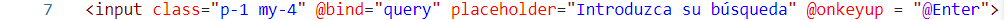
\includegraphics[width=9cm, height=0.2cm]{img02.png}
  \end{figure}
  
  \pause 

  \begin{figure}
    En la línea 32:


    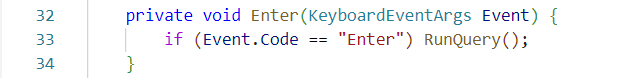
\includegraphics[width=9cm, height=1.2cm]{img01.png}
  \end{figure}

  \end{frame}

\subsection{MoogleEngine}
\begin{frame}[fragile]{MoogleEngine}

  Está compuesta por 8 clases. De ellas hay dos que ya estaban creadas y que no 
  fueron modificadas, que son: \textit{SearchItem} y \textit{Searchresult}.

\pause

\begin{itemize}
\item \textit{Repository:} Es la clase que genera el repositorio de documentos. 
\pause
\item \textit{Document:} Es la clase que tiene los métodos para trabajar con los documentos.
\pause
\item \textit{RankingVector:} Es la clase que contiene el método para asignarle un score a 
cada documento. 
\pause
\item \textit{Operators:} Es la clase que tiene los métodos de los operadores implementados.
\pause 
\item \textit{Moogle:} Es la clase principal del proyecto y donde se generan los resultados de 
las búsquedas. 

\end{itemize}

\end{frame}


